\documentclass[12pt,notitlepage]{article}
\setlength{\parindent}{0pt}
\setlength{\parskip}{6pt}

\usepackage{amsmath}
\usepackage{amsthm}
\usepackage{array}

\usepackage{xunicode}
\usepackage{xltxtra}
\usepackage[table,xcdraw]{xcolor}
\usepackage[shortlabels]{enumitem}
\usepackage{graphicx}
\usepackage[font=scriptsize]{caption}

\usepackage{fourier-otf}
\DeclareMathAlphabet{\mathcal}{OMS}{zplm}{m}{n}

\usepackage[margin=1in,includehead,includefoot,headheight=17pt]{geometry}
\usepackage{fancyhdr}
\pagestyle{fancy}

\usepackage{tikz}
\usepackage{pgfplots}
\pgfplotsset{compat=1.15}

\newcommand{\dd}[1]{\mathop{\mathrm{d}#1}}
\renewcommand{\vec}[1]{\mathbf{#1}}
\newcommand{\curl}{\operatorname{curl}}
\renewcommand{\div}{\operatorname{div}}
\newcommand{\die}{\partial}
\newcommand{\spanvec}{\operatorname{span}}
\newcommand{\range}{\operatorname{range}}
\renewcommand{\null}{\operatorname{null}}
\newcommand{\lcm}{\operatorname{lcm}}
\newcommand{\cis}{\operatorname{cis}}
\newcommand{\sgn}{\operatorname{sgn}}
\newcommand{\Res}{\mathop{\operatorname{Res}}}

\usepackage[many]{tcolorbox}

\definecolor{main}{HTML}{009688} % Main color (light, material teal 500)
% light

\newtcolorbox{thmbox}{
enhanced,
breakable,
boxrule=0pt,frame hidden,
colback=main!10!white,
arc=6pt,
before skip=12pt,after skip=12pt,
boxsep=4pt,
left=6pt,right=6pt,
%sharp corners
}
\newtcolorbox{defbox}{
enhanced jigsaw,
breakable,
boxrule=1.5pt,
colframe=main,
opacityback=0,
arc=6pt,
before skip=12pt,after skip=12pt,
boxsep=4pt,
left=6pt,right=6pt,
%sharp corners
}

\newtcolorbox{exbox}{
enhanced jigsaw,
breakable,
boxrule=0pt,frame hidden,
opacityback=0,
borderline west={1.5pt}{0pt}{main},
before skip=12pt,after skip=12pt,
top=0pt,bottom=0pt,
left=6pt,right=6pt,
sharp corners
}

%\definecolor{main}{HTML}{80CBC4} % Main color (dark, material teal 200)
%% dark

\definecolor{red}{HTML}{EF9A9A}
\definecolor{green}{HTML}{A5D6A7}
\definecolor{blue}{HTML}{90CAF9}
\definecolor{indigo}{HTML}{9FA8DA}
\definecolor{green}{HTML}{A5D6A7}
\definecolor{pink}{HTML}{F48FB1}

\definecolor{darkbg}{HTML}{212121}
\pagecolor{darkbg}
\color{white}

\pgfplotsset{GridPlot1/.style={
    axis lines=center,
    axis line style = thick,
    tick style={thick,white},
    xlabel style={right},
    ylabel style={above},
    grid=both,
    minor tick num=3,
    grid style={line width=.2pt, draw=black!70},
    major grid style={line width=.2pt,draw=gray!50},
}}

\newtcolorbox{thmbox}{
enhanced,
breakable,
boxrule=0pt,frame hidden,
colback=main!15!darkbg,
coltext=white,
arc=6pt,
before skip=12pt,after skip=12pt,
boxsep=4pt,
left=6pt,right=6pt,
%sharp corners
}
\newtcolorbox{defbox}{
enhanced jigsaw,
breakable,
boxrule=1.5pt,
colframe=main,
opacityback=0,
coltext=white,
arc=6pt,
before skip=12pt,after skip=12pt,
boxsep=4pt,
left=6pt,right=6pt,
%sharp corners
}

\newtcolorbox{exbox}{
enhanced jigsaw,
breakable,
boxrule=0pt,frame hidden,
opacityback=0,
coltext=white,
borderline west={1.5pt}{0pt}{main},
before skip=12pt,after skip=12pt,
parbox=false,
top=0pt,bottom=0pt,
left=6pt,right=6pt,
sharp corners
}

\newcommand\bgpic{
    \put(0,0){
    \parbox[b][\paperheight]{\paperwidth}{
    \vfill
    \centering
    \includegraphics[width=\paperwidth,height=\paperheight]{cover_dark.pdf}\vfill
    }}
} % dark mode


\setlist[itemize]{label=\textcolor{main}{\textbullet}}
\setlist[enumerate]{label=\textcolor{main}{\arabic*.}}

\let\oldheadrule\headrule% Copy \headrule into \oldheadrule
\renewcommand{\headrule}{\color{main}\oldheadrule}% Add colour to \headrule
\renewcommand{\headrulewidth}{0.5pt}

\usepackage{titlesec}

\titleformat{\section}
{\color{main}\normalfont\Large\bfseries}
{\color{main}\thesection}{1em}{}

\newtheoremstyle{theoremc} % name
    {}                    % Space above
    {}                    % Space below
    {}                   % Body font \itshape
    {}                           % Indent amount
    {\bfseries\color{main}}                   % Theorem head font
    {.}                          % Punctuation after theorem head
    {.5em}                       % Space after theorem head
    {}

\theoremstyle{theoremc}
\newtheorem{amstheorem}{Theorem}
\numberwithin{amstheorem}{section}
\newtheorem{amsdefinition}{Definition}
\numberwithin{amsdefinition}{section}
\newtheorem{amsexample}{Example}
\numberwithin{amsexample}{section}

\newenvironment{theorem}[1][\unskip]
    {\begin{thmbox}
    \begin{amstheorem}[#1]
    }{\end{amstheorem}
    \end{thmbox}
    }

\newenvironment{definition}[1][\unskip]
    {\begin{defbox}
    \begin{amsdefinition}[#1]
    }{\end{amsdefinition}
    \end{defbox}
    }

\newenvironment{example}[1][\unskip]
    {\begin{exbox}
    \begin{amsexample}[#1]
    }{\end{amsexample}
    \end{exbox}
    }

\lhead{\color{main}STATS 3D03, Fall 2022}
\chead{\color{main}Course Notes by Zach Lucier}
\cfoot{\color{main}\thepage}

\fancypagestyle{plain}{%
\fancyhf{}% clear all header and footer fields
\fancyfoot[C]{\color{main}\thepage} % except the center
\renewcommand{\headrulewidth}{0pt}%
\renewcommand{\footrulewidth}{0pt}%
}

\begin{document}

\rhead{\color{main}1 Review}
\section{Review}

We begin our discussion of mathematical statistics with a review of concepts from previous courses. One of these key concepts is that of probability.

Recall that the \textbf{sample space} $\Omega$ is the set of all possible outcomes of an experiment. Subsets of $\Omega$ are called \textbf{events} and the collection of all events is denoted by $\mathcal F$.

\begin{definition}[probability set function]
	Let $\Omega$ be a sample space and let $\mathcal F$ be the collection of all events. Let $P$ be a real-valued function defined on $\mathcal F$. Then $P$ is a \textbf{probability set function} (also referred to as \textbf{probability measure}, \textbf{probability distribution} or simply \textbf{probability}) if it satisfies the following three conditions:
	\begin{enumerate}
		\item $0\leq P(A)\leq 1$, for all $A\in\mathcal F$.
		\item $P(\Omega)=1$ and $P(\emptyset)$.
		\item If $\{A_n\}$ is a sequence of events in $\mathcal F$ and $A_m\cap A_n=\emptyset$ for all $m\neq n$, then

		$$P\left(\bigcup_{i=1}^\infty A_i\right)=\sum_{i=1}^\infty P(A_i)$$
	\end{enumerate}
\end{definition}

Another important concept is that of a random variable and its support in order to formalize quantities which depend on random events.

\begin{definition}[random variable]
	Let $\Omega$ be a sample space. A \textbf{random variable}, often abbreviated RV, is a function from $\Omega$ into the real numbers. The \textbf{support} (also called \textbf{space} or \textbf{range}) of $X$ is the set of real numbers $\mathcal S=\{x:x=X(\omega),\omega\in \Omega\}$.
\end{definition}

In cases where $\mathcal S$ is a countable set, we say that $X$ is a \textbf{discrete RV}. The set $\mathcal S$ may also be an interval of real numbers, in which case we say that $X$ is a \textbf{continuous RV}.

Given a random variable $X$, its support $\mathcal S$ becomes the sample space of interest. Besides inducing the sample space $\mathcal S$, $X$ also induces a probability which we call the \textbf{distribution} of $X$.

The probability distribution of a discrete random variable is described completely in terms of its probability mass function and its support.

\begin{definition}[pmf]
	Let $X$ be a discrete random variable with support $\mathcal S$. The \textbf{probability mass function} (pmf) of $X$ is given by
$$p_X(x) = P(X = x),\text{ for }x \in \mathcal S.$$
\end{definition}

Similarly, the probability distribution of a continuous random variable is described completely in terms of its probability density function and its support.

\begin{definition}[pdf]
	Let $X$ be a continuous random variable with support $\mathcal S$. The \textbf{probability density function} (pdf) of $X$ is a function $f_X$ that satisfies
$$P(X\in A)=\int_\mathcal Sf_X(x)\dd x$$
where $A$ is a subset of $\mathbb R$ that can be written as a countable union of intervals.
\end{definition}

The pmf of a discrete random variable and the pdf of a continuous random variable are quite different entities. The cumulative distribution function, though, uniquely determines the probability distribution of a random variable.

\begin{definition}[cdf]
	Let $X$ be a random variable. Then its \textbf{cumulative distribution function} (cdf) is defined by $F_X(x)$, where
$$F_X(x)=P(X\leq x).$$
\end{definition}

One of the most important measures associated with RVs is that of expectation.

\begin{definition}[expectation]
	Let $X$ be a random variable with support $\mathcal S$.

	If $X$ is a \textit{continuous} random variable with pdf $f(x)$ and
	$$\int_{\mathcal S}|x|f(x)\dd x$$
	is finite, then the \textbf{expectation} of $X$, denoted $E(X)$ is defined as
	$$E(X)=\int_{\mathcal S} xf(x)\dd x.$$ 

	If $X$ is a \textit{discrete} random variable with pmf $p(x)$ and
	$$\sum_{x\in\mathcal S}|x|p(x)$$
	is finite, then the \textbf{expectation} of $X$ is defined as
	$$\sum_{x\in\mathcal S}xp(x).$$
\end{definition}

Sometimes the expectation $E(X)$ is called the \textbf{expected value} of $X$ or the \textbf{mean} of $X$. When the mean designation is used, we often denote the expected value by $\mu$.

\begin{theorem}[]
	Let $X$ be a random variable and let $Y=g(X)$ for some function $g$.
	\begin{enumerate}[label=\color{main}(\alph*)]
		\item Suppose $X$ is discrete with pmf $p_X(x)$ and support $\mathcal S_X$. If $\sum_{x\in\mathcal S_X}|g(x)|p_X(x)$ is finite, then the expectation of $Y$ exists and is given by $$\sum_{x\in\mathcal S_X}g(x)p_X(x).$$
		\item Suppose $X$ is continuous with pdf $f_X(x)$ and support $\mathcal S_X$. If $\int_{\mathcal S_X}|g(x)|f_X(x)\dd x$ is finite, then the expectation of $Y$ exists and is given by $$\int_{\mathcal S_X}g(x)f_X(x)\dd x.$$
	\end{enumerate}
\end{theorem}

An important application of the above theorem shows that expectation is \textit{linear}. That is, $E(aX+b)=aE(X)+b$. Furthermore, this property can be generalized for $a_1,\hdots,a_k$ real numbers and $g_1,\hdots,g_k$ real-valued functions.
$$E(a_1g_1(X)+\cdots+a_kg_k(X))=a_1E(g_1(X))+\cdots+a_kE(g_k(X))$$

Expectation allows us to define a countably infinite number of measures associated with RVs, called moments.

\begin{definition}[moment]
	Suppose $X$ is a RV and $m$ is a positive integer. The \textbf{$m$th moment} of $X$ is defined to be $E(X^m)$, provided this expectation exists.
\end{definition}

As such, the 1st moment of a RV is simply its \textbf{mean} $\mu$. It is often useful to think about moments about the mean $E((X-\mu)^m)$. We call these \textbf{central moments}. The 2nd central moment should be familiar to you as the \textbf{variance} $\sigma^2$. We call the 3rd central moment the \textbf{skewness} and call the 4th central moment the \textbf{kurtosis}.

\begin{definition}[moment generating function]
	Let $X$ be a random variable such that for some $h>0$, the expectation of $e^{tX}$ exists for $-h<t<h$. The \textbf{moment generating function} of $X$ is defined to be the function $M_X(t)=E(e^{tX})$ for $-h<t<h$.
\end{definition}

Clearly, $M_X(0)=1$ for any RV. Not every random variable has a mgf. For example, the mgf of the Cauchy Distribution with pdf $f(x)=\frac{1}{\pi(1+x^2)}$ is not defined. It can be shown that if the mgf of a RV exists, then all of its moments exist.

\begin{theorem}[]
	Let $X$ and $Y$ be RVs with mgfs $M_X$ and $M_Y$, respectively, existing in open intervals about 0. Then $F_X(z)=F_Y(z)$ for all $z\in\mathbb R$ if and only if $M_X(t)=M_Y(t)$ for all $t\in(-h,h)$ for some $h>0$.
\end{theorem}

\begin{theorem}[]
	Let $X$ be a RV with mgf $M_X$, and let $a,b\in\mathbb R$ be fixed. Then the mgf of $Y=aX+b$ also exists and is given by $$M_Y(t)=e^{bt}M_X(at).$$
\end{theorem}

\begin{theorem}[]
	Suppose $X$ and $Y$ are independent RVs with mgfs $M_X$ and $M_Y$. Let $a,b\in\mathbb R$ be fixed and define $Z+aX+bY$. Then the mgf of $Z$ exists in an open interval about 0 and is given by
	$$M_Z(t)=M_X(at)M_Y(bt).$$
\end{theorem}

\begin{theorem}[]
	Suppose $X$ is a RV with mgf $M_X$ and $M_X^{(m)}(t)=\frac{\mathrm{d}^m}{\dd t^m}M_X(t)$. Then the $m$th moment of $X$ is given by $$E(X^m)=M_X^{(m)}(0).$$
\end{theorem}

The above theorem should make clear why we call mgfs as such. The proof is reliant on the Taylor expansion of $e^{tX}$. Observe the following.
\begin{align*}
	M_X(t)&=E(e^{tX})\\
	&=E\left(\sum_{n=0}^\infty \frac{t^n}{n!}X^n\right)\\
	&=\sum_{n=0}^\infty \frac{t^n}{n!}E(X^n)
\end{align*}

We reintroduce some special distributions, starting with those of the discrete kind.

\begin{definition}[binomial RV]
	Assume a sequence of $n$ Bernouilli trials each with probability of success $p$ and let $X$ be the number of successes. Then $X$ is a \textbf{binomial RV} with pmf $$p_X(x)=\begin{cases}
		\binom{n}{x}p^x(1-p)^{n-x} & \text{for $x=0,1,\hdots,n$}\\
		0 & \text{otherwise}
	\end{cases}$$
	We write $X\sim b(n,p)$.
\end{definition}

If $X\sim b(n,p)$, $X$ has support $\{0,1,\hdots,n\}$, mean $\mu=np$, variance $\sigma^2=np(1-p)$ and mgf $M_X(t)=(1-p+pe^t)^n$.

\begin{definition}[negative binomial RV]
	Assume a sequence of Bernouilli trials each with probability of success $p$ is performed until the $r$th success occurs. Let $Y$ be the number of trials required. Then $Y$ is a \textbf{negative binomial RV} with pmf $$p_Y(y)=\begin{cases}
		\binom{y+r-1}{y-1}p^r(1-p)^y & \text{for $y=0,1,\hdots$}\\
		0 & \text{otherwise}
	\end{cases}$$
	We write $Y\sim \mathop{nb}(r,p)$.
\end{definition}

If $Y\sim \mathop{nb}(r,p)$, $Y$ has support $\mathbb Z_{\geq 0}$, mean $\mu=\frac{pr}{1-p}$, variance $\sigma^2=\frac{pr}{(1-p)^2}$ and mgf $M_Y(t)=\left(\frac{1-p}{1-pe^t}\right)$ with $t<-\ln p$.

Taking $r=1$, we obtain the geometric distribution.

\begin{definition}[Poisson RV]
	A discrete RV $X$ is a \textbf{Poisson RV} if its pmf has the form $$p_X(x)=\begin{cases}
		\frac{\lambda^xe^{-\lambda}}{x!} & \text{for $x=0,1,\hdots$}\\
		0 & \text{otherwise}
	\end{cases}$$
	where $\lambda\in\mathbb R_{\geq 0}$. We write $X\sim \operatorname{Pois}(\lambda)$.
\end{definition}

If $X\sim \operatorname{Pois}(\lambda)$, $X$ has support $\mathbb Z_{\geq 0}$, mean $\mu=\lambda$, variance $\sigma^2=\lambda$ and mgf $M_X(t)=\exp(\lambda(e^t-1))$.

We now recall some continuous distributions.

\begin{definition}[uniform RV]
	A continuous RV $X$ is said to be a \textbf{uniform RV} if it has pdf
	$$p_X(x)=\begin{cases}
		\frac{1}{b-a} & \text{for $x\in[a,b])$}\\
		0 & \text{otherwise}
	\end{cases}$$
	where $a,b\in\mathbb R$ are fixed. We write $X\sim U(a,b)$.
\end{definition}

If $X\sim U(a,b)$, $X$ has support $[a,b]$, mean $\mu=\frac{a+b}{2}$, variance $\sigma^2=\frac{(b-a)^2}{12}$ and mgf $M_X(t)=\begin{cases}
	\frac{e^{tb}-e^{ta}}{t(b-a)} & \text{for $t\neq 0$}\\
	1 & \text{for $t= 0$}
\end{cases}$.

\begin{definition}[normal RV]
	A continuous RV $X$ is said to be a \textbf{normal RV} with parameters $\mu\in\mathbb R$ and $\sigma^2>0$ if its pdf has the form
	$$f_X(x)=\frac{1}{\sqrt{2\pi}\sigma}e^{-\frac{(x-\mu)^2}{2\sigma^2}}.$$
	We write $X\sim N(\mu,\sigma^2)$.
\end{definition}

If $X\sim N(\mu,\sigma^2)$, $X$ has support $\mathbb R$, mean $\mu$, variance $\sigma^2$ and mgf $M_X(t)=e^{\mu t+\frac{\sigma^2 t^2}{2}}$.

The derivation of this mgf follows, as a review.

\begin{align*}
	M_X(t)&=E(e^{tX})\\
	&=\int_{-\infty}^\infty\frac{1}{\sqrt{2\pi}\sigma}e^{-\frac{(x-\mu)^2}{2\sigma^2}}e^{tx}\dd x\\
	\intertext{Let $z=\frac{x-\mu}{\sigma}$.}
	&=e^{\mu t}\int e^{z\sigma t}\frac 1{\sqrt{2\pi\sigma^2}}e^{-\frac 12z^2}\dd z\\
	&=e^{\mu t}e^{\frac{\sigma^2 t^2}{2}}\\
	&=e^{\mu t+\frac{\sigma^2 t^2}{2}}
\end{align*}

\begin{theorem}[]
	Let $X_1,\hdots,X_n$ be IID RVs such that $X_i\sim N(\mu_i,\sigma_i^2)$ for each $i=1,\hdots,n$. Let $Y=\sum_{i=1}^na_iX_i$ for some set of real constants $\{a_1,\hdots,a_n\}$. Then $Y$ is also normally distributed and
$$Y\sim N\left(\sum_{i=1}^na_i\mu_i,\sum_{i=1}^na_i^2\sigma_i^2\right).$$
\end{theorem}

\begin{definition}[gamma RV]
	A continuous RV $X$ is said to be a \textbf{gamma RV} with parameters $\alpha,\beta>0$ if its pdf has the form
	$$f_X(x)=\begin{cases}
		\frac{\beta^\alpha}{\Gamma(\alpha)} x^{\alpha - 1} e^{-\beta x } & \text{for $x\in\mathbb R_{>0}$}\\
		0 & \text{otherwise}
	\end{cases}.$$
	We write $X\sim \Gamma(\alpha,\beta)$.
\end{definition}

Taking $\alpha=1$ yields the exponential distribution.

If $X\sim \Gamma(\alpha,\beta)$, $X$ has support $\mathbb R_{>0}$, mean $\mu=\frac{\alpha}{\beta}$, variance $\sigma^2=\frac{\alpha}{\beta^2}$ and mgf $M_X(t)=\left(1 - \frac{t}{\beta}\right)^{-\alpha}$ for $t < \beta$.


\begin{definition}[beta RV]
	A continuous RV $X$ is said to be a \textbf{beta RV} with parameters $\alpha,\beta>0$ if its pdf has the form
	$$f_X(x)=\begin{cases}
		\frac{x^{\alpha-1}(1-x)^{\beta-1}} {\mathrm{B}(\alpha,\beta)} & \text{for $x\in(0,1)$}\\
		0 & \text{otherwise}
	\end{cases}$$
	where $\mathrm{B}(\alpha,\beta) = \frac{\Gamma(\alpha)\Gamma(\beta)}{\Gamma(\alpha + \beta)}$. We write $X\sim \operatorname{Beta}(\alpha,\beta)$.
\end{definition}

If $X\sim \operatorname{Beta}(\alpha,\beta)$, $X$ has support $(0,1)$, mean $\mu=\frac{\alpha}{\alpha + \beta}$, variance $\sigma^2=\frac{\alpha\beta}{(\alpha+\beta)^2(\alpha+\beta+1)}$ and mgf $M_X(t)=1+\sum_{k=1}^{\infty} \left( \prod_{r=0}^{k-1} \frac{\alpha+r}{\alpha+\beta+r} \right) \frac{t^k}{k!}$.


\break

\rhead{\color{main}2 Multivariate distributions}
\section{Multivariate distributions}

We will often want to deal with more than one variable based on the same random experiment.

\begin{definition}[random vector]
	Consider a random experiment with sample space $\Omega$. Let $X_1,X_2:\Omega\to\mathbb R$ be random variables. We say that $(X_1,X_2)$ is a \textbf{random vector}. The support of $(X_1,X_2)$ is the set of ordered pairs $\chi=\{(x_1,x_2):X_1(\omega)=x_1,X_2(\omega)=x_2,\omega\in \Omega\}$.
\end{definition}

Of particular interest are events of the forms $(X_1\leq x_1)\cap(X_2\leq x_2)$ for $(x_1,x_2)\in\mathbb R^2$.

\begin{definition}[joint cdf]
	Suppose that $(X_1,X_2)$ is a random vector. The \textbf{joint cdf} is defined as $$F_{X_1,X_2}(x_1,x_2)=P((X_1\leq x_1)\cap(X_2\leq x_2)).$$
\end{definition}

From here we can extend the univariate case for the probability over intervals to rectangular subsets of $\mathbb R^2$.

\begin{theorem}[]
	Suppose that the random vector $(X_1,X_2)$ has joint cdf $F_{X_1,X_2}$ and let $a_1,b_1,a_2,b_2\in\mathbb R$ be such that $a_1<b_1$ and $a_2<b_2$. Then $$P((X_1,X_2)\in[a_1,b_1]\times[a_2,b_2])=F_{X_1,X_2}(b_1,b_2)-F_{X_1,X_2}(a_1,b_2)-F_{X_1,X_2}(b_1,a_2)+F_{X_1,X_2}(a_1,a_2).$$
\end{theorem}

Recall that, in general, random variables can be of the discrete type or of the continuous type. We extend this idea to random vectors.

A random vector $(X_1,X_2)$ is said to be \textbf{discrete} if its support $\chi$ is countable. In this case both $X_1$ and $X_2$ are discrete random variables. It thus makes sense to define pmfs for random vectors.

\begin{definition}[joint pmf]
	Let $(X_1,X_2)$ be a discrete random vector. Then the \textbf{joint pmf} of $(X_1,X_2)$ is given by

	$$p_{X_1,X_2}(x_1,x_2)=P(X_1=x_1,X_2=x_2).$$
\end{definition}

As in the univariate case, this joint pmf satisfies the following properties.
\begin{enumerate}
	\item $0\leq p_{X_1,X_2}(x_1,x_2)\leq 1$ for all $(x_1,x_2)\in\chi$.
	\item $\sum_{(x_1,x_2)\in\chi}p_{X_1,X_2}(x_1,x_2)=1$.
\end{enumerate}

\begin{example}[]
	Suppose two dice are rolled. Let $X$ denote the number of dots facing up on the first die and $Y$ the number of dots on the second die. Also, let $W=\max(X,Y)$. We would like to find the joint pmf of the random vector $(X,W)$ and the probability that $X=W$.

	\textit{Solution.} Let $\chi$ denote the support of $(X,W)$. It is clear that $\chi=\{1,\hdots,6\}\times\{1,\hdots,6\}$.

	By the equally likely model, the joint pmf $p_{X,W}$ of $(X,W)$ can be summarized by the following table.

	\begin{center}
	%\rowcolors{2}{white}{main!10}
	\begin{tabular}{c | c c c c c c}
		$W/X$ & 1 & 2 & 3 & 4 & 5 & 6\\\hline
		1 & $\frac{1}{36}$ & 0 & 0 & 0 & 0 & 0\\
		2 & $\frac{1}{36}$ & $\frac{2}{36}$ & 0 & 0 & 0 & 0\\
		3 & $\frac{1}{36}$ & $\frac{1}{36}$ & $\frac{3}{36}$ & 0 & 0 & 0\\
		4 & $\frac{1}{36}$ & $\frac{1}{36}$ & $\frac{1}{36}$ & $\frac{4}{36}$ & 0 & 0\\
		5 & $\frac{1}{36}$ & $\frac{1}{36}$ & $\frac{1}{36}$ & $\frac{1}{36}$ & $\frac{5}{36}$ & 0\\
		6 & $\frac{1}{36}$ & $\frac{1}{36}$ & $\frac{1}{36}$ & $\frac{1}{36}$ & $\frac{1}{36}$ & $\frac{6}{36}$
	\end{tabular}
	\end{center}

	It is clearly the case that $0\leq p_{X,W}(x,w)\leq 1$ and $\sum_{(x,w)\in(X,W)}p_{X,W}(x,w)=1$.

	We can now find the probability that $X=W$. That is, that the first die has the larger number of dots. We sum along the diagonal of the above table.
	\begin{align*}
		\sum_{\substack{(x,w)\in\chi\\x=w}}p_{X,W}(x,w)&=\frac 1{36}+\frac{2}{36}+\cdots+\frac{6}{36}\\
		&=\frac{7}{12}
	\end{align*}

\end{example}

If the joint cdf $F_{X_1,X_2}$ of a random vector $(X_1,X_2)$ is continuous, then we say that $(X_1,X_2)$ is \textbf{continuous}. Similarly to a joint pmf, we can also define a joint pdf.

\begin{definition}[joint pdf]
	Let $(X_1,X_2)$ be a continuous random vector. Then the \textbf{joint pdf} of $(X_1,X_2)$ is the function $f_{X_1,X_2}:\mathbb R^2\to\mathbb R_{>0}$ satisfying
	$$F_{X_1,X_2}(x_1,x_2)=\int_{-\infty}^{x_2}\int_{-\infty}^{x_1}f_{X_1,X_2}(u,v)\dd u\dd v$$
	for all $(x_1,x_2)\in\mathbb R^2$.
\end{definition}

As in the univariate case, the joint pdf satisfies the following properties.
\begin{enumerate}
	\item $f_{X_1,X_2}(x_1,x_2)\geq 0$ for all $(x_1,x_2)\in\mathbb R^2$.
	\item $\int_{-\infty}^{\infty}\int_{-\infty}^{\infty}f_{X_1,X_2}(u,v)\dd u\dd v=1$.
\end{enumerate}

Often times, we will want to obtain the distributions of the random variables $X_1$ and $X_2$ from the joint distribution of $(X_1,X_2)$.

Given the above setup, we obtain the \textbf{marginal cdf} from the following equivalent formulations.
\begin{align*}
	F_{X_1}&=P(X_1\leq x_1)\\
	&=P(X_1\leq x_1,-\infty<X_2<\infty)\\
	&=\lim_{x_2\to\infty}P(X_1\leq x_1,X_2\leq x_2)\\
	&=\lim_{x_2\to\infty} F_{X_1,X_2}(x_1,x_2)
\end{align*}

We may also find \textbf{marginal pmfs} and \textbf{marginal pdfs}.

If $(X_1,X_2)$ is a discrete random vector, then
\begin{align*}
	p_{X_1}(x_1)&=P(X_1=x_1)\\
	&=\sum_{x_2}p_{X_1,X_2}(x_1,x_2)
\end{align*}

If $(X_1,X_2)$ is a continuous random vector, then
\begin{align*}
	f_{X_1}(x_1)&=\int_{-\infty}^{\infty}f_{X_1,X_2}(x_1,x_2)\dd{x_2}\\
\end{align*}

\begin{example}[]
	We revisit the previous example. We would like to find the marginal pmf of $W$.

	\textit{Solution.} We apply the definition.
	\begin{center}
	\begin{tabular}{c | c}
		$W$ & $p_W(w)$\\ \hline
		1 & $\frac{1}{36}$\\
		2 & $\frac{3}{36}$\\
		3 & $\frac{5}{36}$\\
		4 & $\frac{7}{36}$\\
		5 & $\frac{9}{36}$\\
		6 & $\frac{11}{36}$
	\end{tabular}
	\end{center}
\end{example}


\begin{example}[]
	Consider the joint pdf of $(X,Y)$ to be
	$$f_{X,Y}(x,y)=\begin{cases}
		cxy^2 & \text{for $0\leq x\leq 2,0\leq y\leq 1$}\\
		0 & \text{otherwise}
	\end{cases}$$
	We would like to find the value of $c$ such that $f_{X,Y}$ is a valid pdf. We would then like to find the marginal pdfs.

	For $f_{X,Y}$ to be valid, we require it to be non-negative and it must integrate to 1. The second property will be used to determine $c$.

	\begin{align*}
		\int_0^1\int_0^2 cxy^2\dd x\dd y & =1\\
		c\int_0^1y^2\int_0^2 x\dd x\dd y & =1\\
		c\left(\frac 13\right)(2)&=1\\
		\frac 23 c&=1\\
		c&=\frac 32
	\end{align*}

	Such a $c$ makes $f_{X,Y}$ a valid pdf.

	We first find the marginal pdf of $X$.

	\begin{align*}
		f_X(x)&=\int_0^1\frac 32xy^2\dd y\\
		&=\frac 32x\int_0^1y^2\dd y\\
		&=\frac x2
	\end{align*}

	So $f_X(x)=\begin{cases}
		\frac x 2 & \text{for $0\leq x\leq 2$}\\
		0 & \text{otherwise}
	\end{cases}$

	We leave the marginal pdf of $Y$ as an exercise.
\end{example}

Expectations in the multivariate case are easily extended from the univariate case to random vectors.

Suppose $(X_1,X_2)$ is a random vector and let $Y=g(X_1,X_2)$ for $g:\mathbb R^2\to\mathbb R$.

If $(X_1,X_2)$ is discrete with joint pmf $p_{X_1,X_2}$, then $E(Y)$ exists if [insert condition] and is defined as $$E(Y)=\sum_{x_1}\sum_{x_2} g(x_1,x_2)p_{X_1,X_2}(x_1,x_2)$$


\end{document}